\documentclass[a4paper,12pt]{article}

\usepackage{xifthen}
\usepackage{xparse}
\usepackage{dsfont}
\usepackage{amsthm}
\usepackage{amssymb}
\usepackage{amsmath}


% Left-right bracket
\newcommand{\lr}[1]{\left (#1\right)}

% Left-right square bracket
\newcommand{\lrs}[1]{\left [#1 \right]}

% Left-right curly bracket
\newcommand{\lrc}[1]{\left \{#1\right\}}

% Left-right absolute value
\newcommand{\lra}[1]{\left |#1\right|}

% Left-right upper value
\newcommand{\lru}[1]{\left \lceil#1\right\rceil}

% Scalar product
\newcommand{\vp}[2]{\left \langle #1 , #2 \right \rangle}

% The real numbers
\newcommand{\R}{\mathbb R}

% The natural numbers
\newcommand{\N}{\mathbb N}

% Expectation symbol with an optional argument
\NewDocumentCommand{\E}{o}{\mathbb E\IfValueT{#1}{\lrs{#1}}}

% Indicator function with an optional argument
\NewDocumentCommand{\1}{o}{\mathds 1{\IfValueT{#1}{\lr{#1}}}}

% Probability function
\let\P\undefined
\NewDocumentCommand{\P}{o}{\mathbb P{\IfValueT{#1}{\lr{#1}}}}

% A hypothesis space
\newcommand{\HH}{\mathcal H}

% A sample space
\newcommand{\XX}{\mathcal{X}}

% A label space
\newcommand{\YY}{\mathcal{Y}}

% A nicer emptyset symbol
\let\emptyset\varnothing

% Sign operator
\DeclareMathOperator{\sign}{sign}
\newcommand{\sgn}[1]{\sign\lr{#1}}

% KL operator
\DeclareMathOperator{\KL}{KL}

% kl operator
\DeclareMathOperator{\kl}{kl}

% kl upper inverse operator
\DeclareMathOperator{\klui}{kl^{-1^+}\!}


% The entropy
\let\H\relax
\DeclareMathOperator{\H}{H}

% Majority vote
\DeclareMathOperator{\MV}{MV}

% Variance
\DeclareMathOperator{\V}{Var}
\NewDocumentCommand{\Var}{o}{\V\IfValueT{#1}{\lrs{#1}}}

% VC
\DeclareMathOperator{\VC}{VC}

% VC-dimension
\newcommand{\dVC}{d_{\VC}}

% FAT ...
\DeclareMathOperator{\FAT}{FAT}
\newcommand{\dfat}{d_{\FAT}}
\newcommand{\lfat}{\ell_{\FAT}}
\newcommand{\Lfat}{L_{\FAT}}
\newcommand{\hatLfat}{\hat L_{\FAT}}

% Distance
\DeclareMathOperator{\dist}{dist}


\usepackage{a4wide}
\usepackage{amsfonts}
\usepackage{amsmath}
\usepackage{amssymb}
\usepackage{lipsum}
\usepackage{amsthm}

\usepackage{graphicx}  % For including images

\usepackage{xcolor}  % For a colorfull presentation
\usepackage{listings}  % For presenting code 

\usepackage{hyperref}

\newtheorem{theorem}{Theorem}
\newtheorem{lemma}[theorem]{Lemma}
\newtheorem{corollary}[theorem]{Corollary}

\setlength\parindent{0pt}

% Definition of a style for code, matter of taste
\lstdefinestyle{mystyle}{
  language=Python,
  basicstyle=\ttfamily\footnotesize,
  backgroundcolor=\color[HTML]{F7F7F7},
  rulecolor=\color[HTML]{EEEEEE},
  identifierstyle=\color[HTML]{24292E},
  emphstyle=\color[HTML]{005CC5},
  keywordstyle=\color[HTML]{D73A49},
  commentstyle=\color[HTML]{6A737D},
  stringstyle=\color[HTML]{032F62},
  emph={@property,self,range,True,False},
  morekeywords={super,with,as,lambda},
  literate=%
    {+}{{{\color[HTML]{D73A49}+}}}1
    {-}{{{\color[HTML]{D73A49}-}}}1
    {*}{{{\color[HTML]{D73A49}*}}}1
    {/}{{{\color[HTML]{D73A49}/}}}1
    {=}{{{\color[HTML]{D73A49}=}}}1
    {/=}{{{\color[HTML]{D73A49}=}}}1,
  breakatwhitespace=false,
  breaklines=true,
  captionpos=b,
  keepspaces=true,
  numbers=none,
  showspaces=false,
  showstringspaces=false,
  showtabs=false,
  tabsize=4,
  frame=single,
}
\lstset{style=mystyle}

\begin{document}
\title{Machine Learning B (2025)\\Home Assignment 1}
\author{\color{red}Carsten Jørgensen, student ID: skj730}
\date{}
\maketitle

% Please leave the table of contents as is, for the ease of navigation for TAs
\tableofcontents % Generates the table of contents
\newpage % Start a new page after the table of contents

\section{Numerical comparison of \texorpdfstring{$\kl$}{kl} inequality with its relaxations and with Hoeffding's inequality (40 points) [Yevgeny]}

\subsection*{Bounds}
We shall evaluate the following four bounds on $p$:

\begin{itemize}
    \item Hoeffding: $\hat{p}_n + \sqrt{\frac{\ln \frac{1}{\delta}}{2n}}$
    \item The $\kl$ inequality: $\kl^{-1^+} (\hat{p}_n, \epsilon) = \max \{ p : \mathrm{kl} (\hat{p}_n\|p) \leq \epsilon \}$
    \item Pinsker’s relaxation: identical to Hoeffding according to eq. (2.12) in the lecture notes
    \item Refined Pinsker’s: $\hat{p}_n + \sqrt{\frac{2\hat{p}_n\ln \frac{1}{\delta} }{n}} + \frac{2\ln \frac{1}{\delta} }{n} $
\end{itemize}

\subsection*{Plot of upper bounds}
In figure \ref{fig:upper_bounds} we plot the upper bounds. 
\begin{center}
    \begin{figure}[ht]
        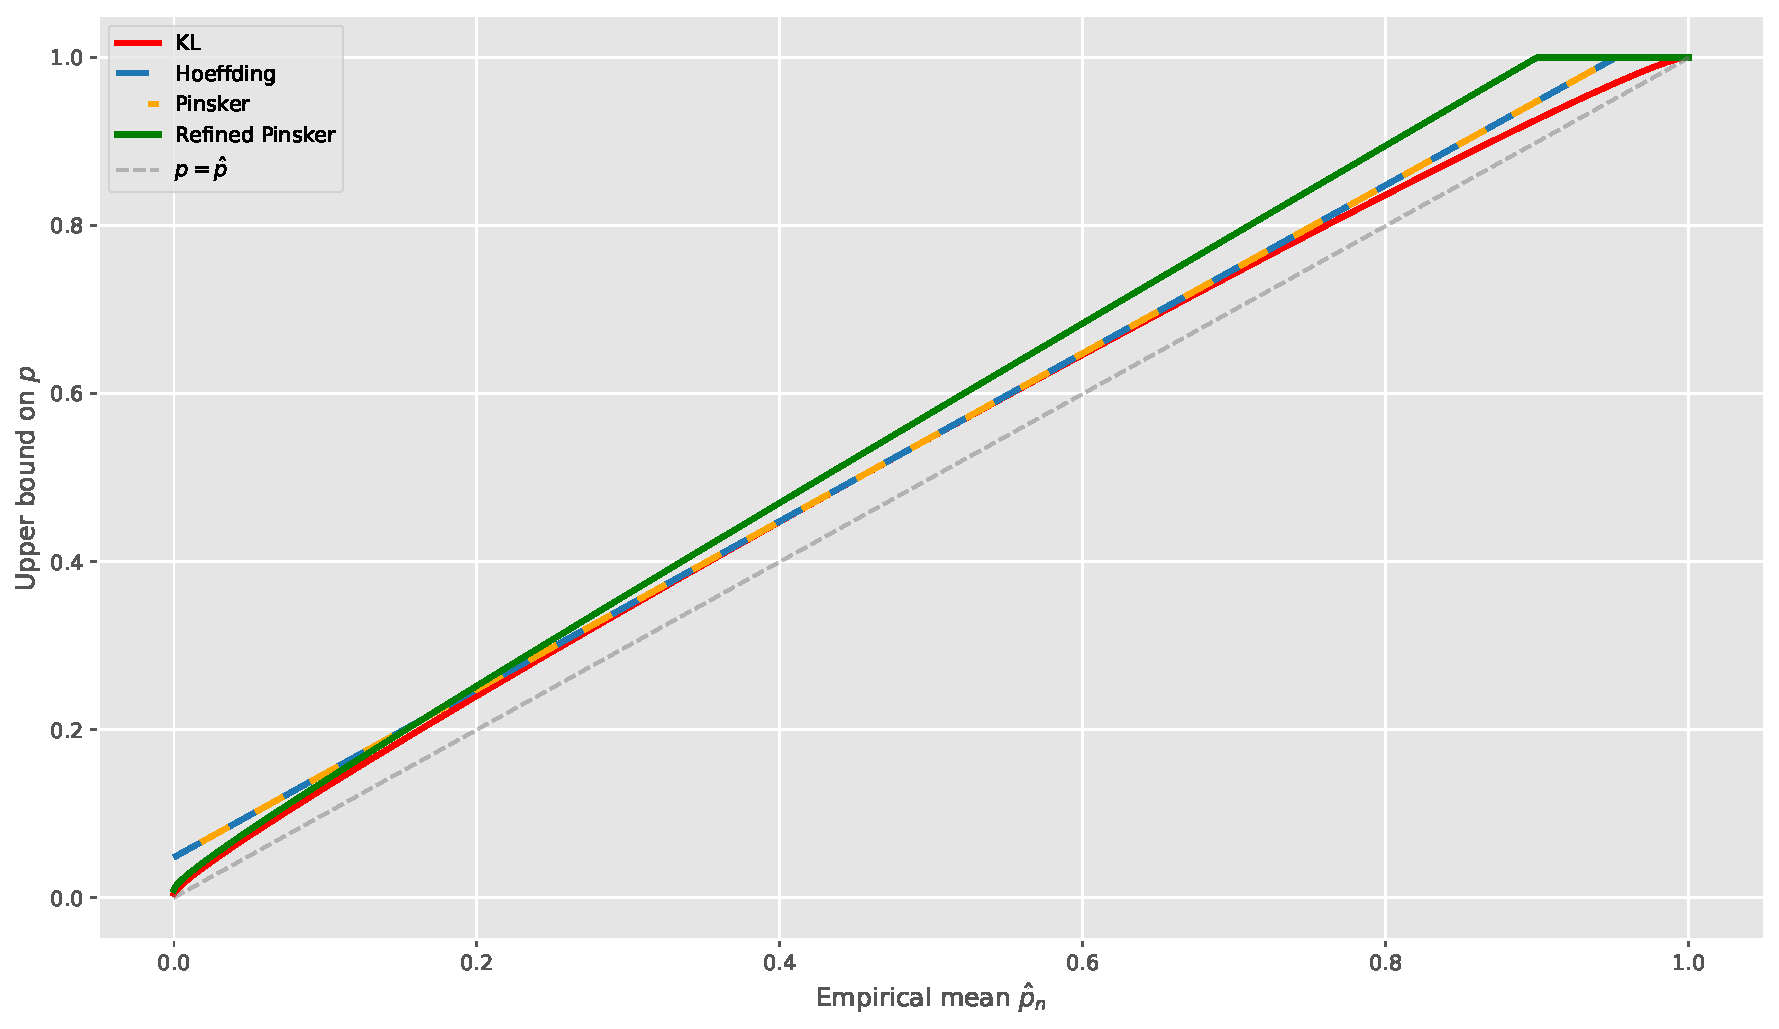
\includegraphics[scale=0.53]{figures/upper_bounds.pdf}
        \caption{Upper bounds for $\hat{p}_n \in [0,1]$}
        \label{fig:upper_bounds}
    \end{figure}
\end{center}
and in figure \ref{fig:zoomed_upper_bounds} we plot the same upper bounds "zoomed in" on $\hat{p}_n \in [0,0.1]$.
\begin{center}
    \begin{figure}[ht]
        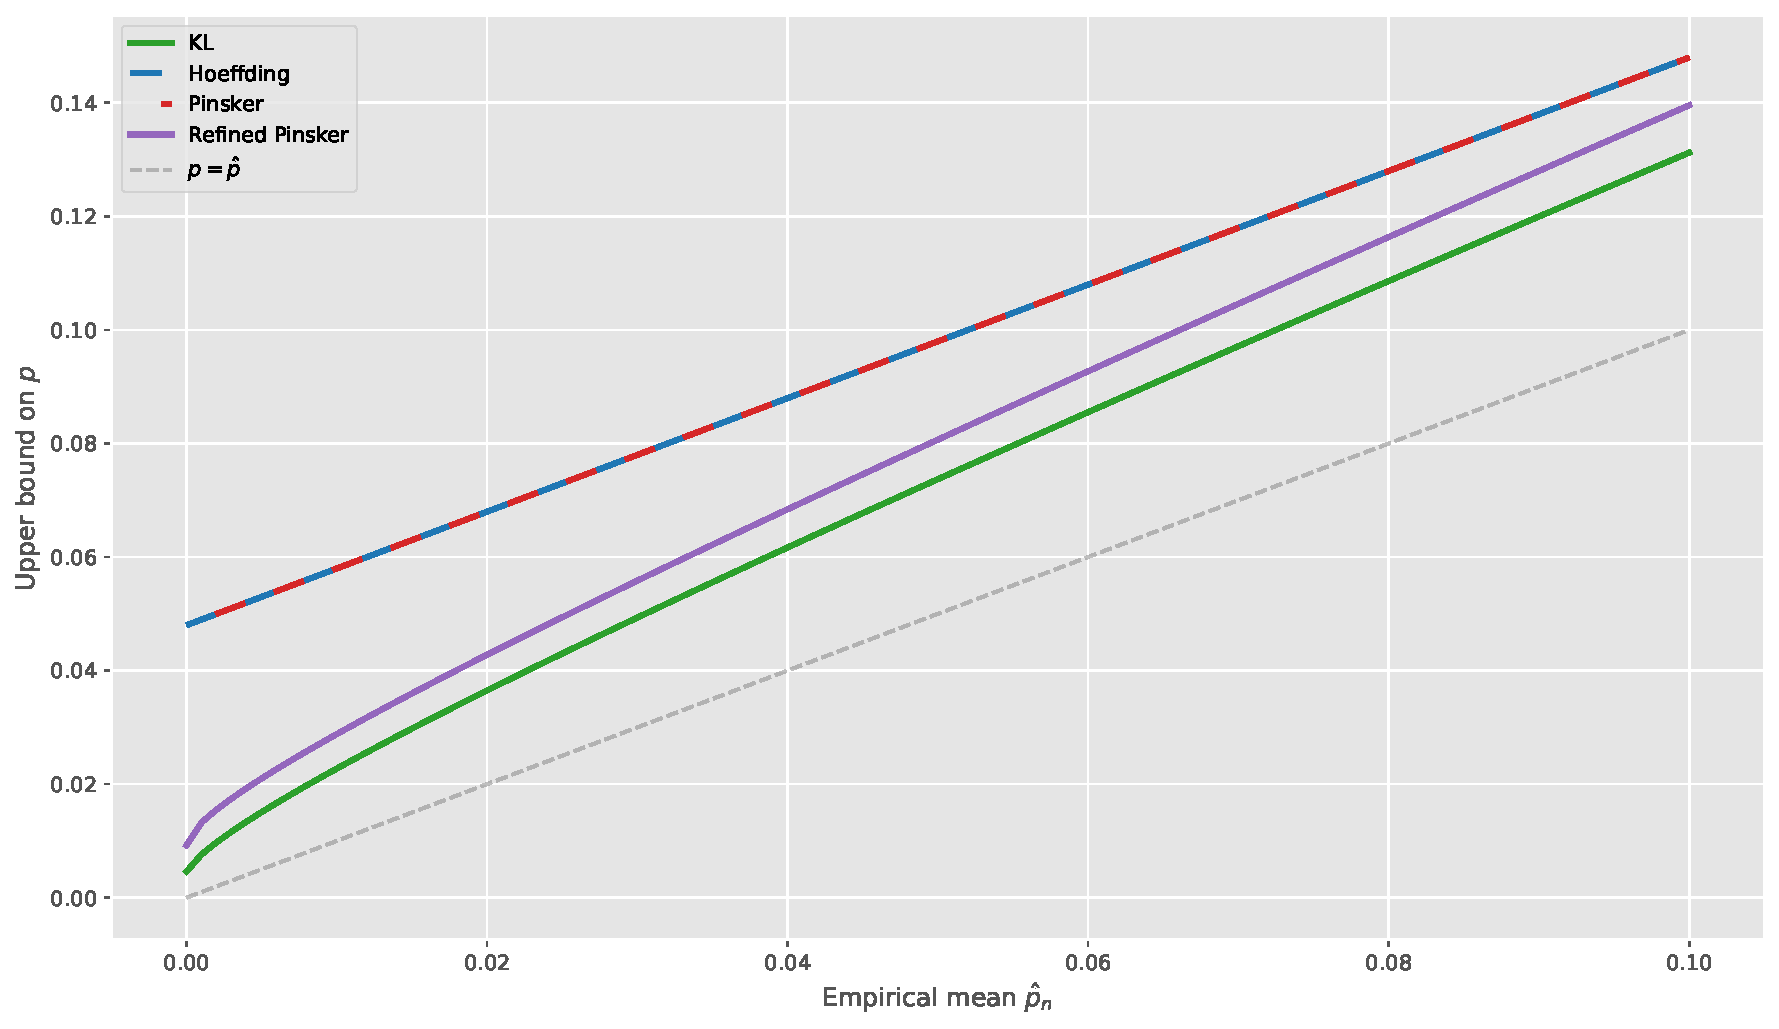
\includegraphics[scale=0.53]{figures/zoomed_in_upper_bounds.pdf}
        \caption{Zoomed upper bounds for $\hat{p}_n \in [0,0.1]$}
        \label{fig:zoomed_upper_bounds}
    \end{figure}
\end{center}

\subsection*{Plot of lower bounds}
The lower bounds are shown in figure \ref{fig:lower_bounds}.
\begin{center}
    \begin{figure}[ht]
        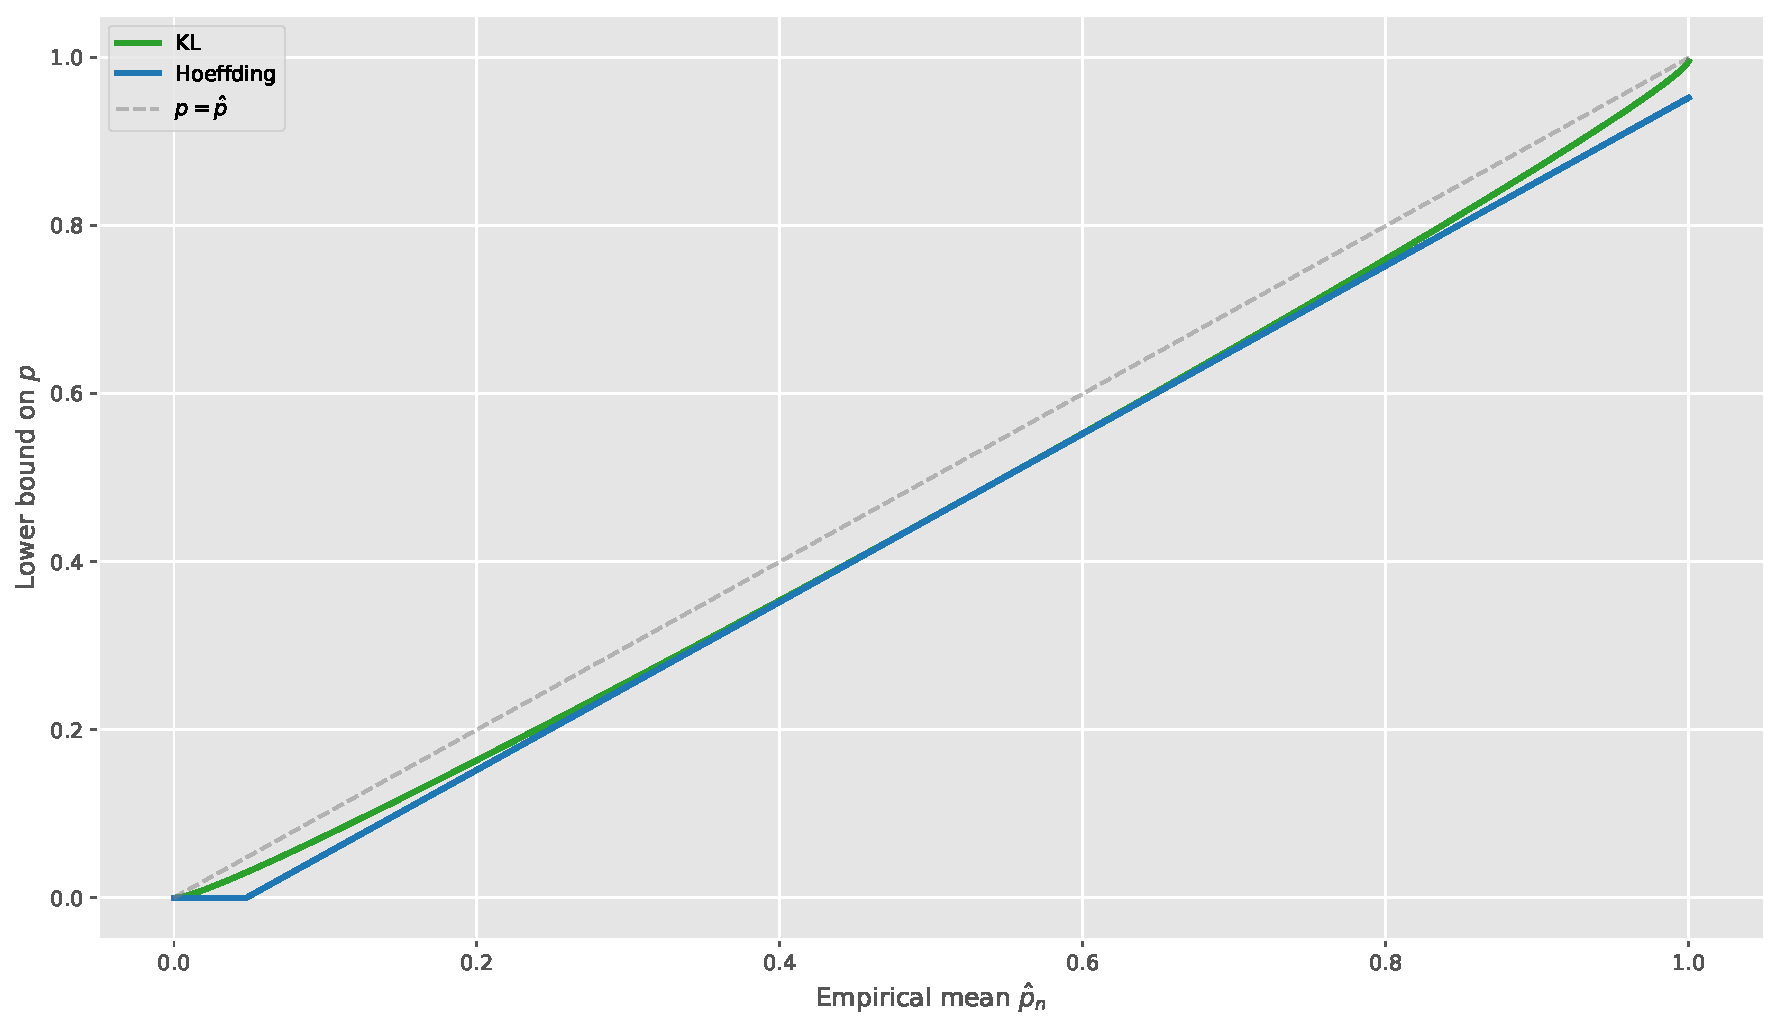
\includegraphics[scale=0.53]{figures/lower_bounds.pdf}
        \caption{Lower bounds for $\hat{p}_n \in [0,1]$}
        \label{fig:lower_bounds}
    \end{figure}
\end{center}

\subsection*{Computation of upper and lower inverse of $\kl$}
Please see \ref{lst:upper_inverse} for the implementation of the upper inverse of $\kl$. To compute the lower inverse of $\kl$, we note that $\kl(a\|b)=\kl(1-a\|1-b)$ for all $a,b \in [0,1]$. So $\kl(\hat{p}\|p) \leq \epsilon$ is equivalent to $\kl(1-\hat{p}\|1-p) \leq \epsilon$. For $q=1-p$ the sets ${p : \kl(\hat{p}\|p) \leq \epsilon}$ and ${q : \kl(1-\hat{p}\|q) \leq \epsilon}$ are identical.
\\[2mm]
By the definition of the upper inverse we have 
\begin{equation*}
    q^+ = \kl^{-1^+} (1-\hat{p}, \epsilon) = \max \{q \geq 1-\hat{p} : \kl(1-\hat{p}\|q) \leq \epsilon \}
\end{equation*}
We now replace $q$ with $1-p$ to obtain
\begin{equation*}
    p^- = 1-q^+ = 1-  \kl^{-1^+} (1-\hat{p}, \epsilon) = \min \{p \leq \hat{p}  : \kl(\hat{p}\|p) \leq \epsilon \} = \kl^{-1^-}(\hat{p}, \epsilon )
\end{equation*}
So the lower inverse can be obtained from the upper inverse through the code:
\lstinputlisting[caption=Lower inverse, label={lst:lower_inverse}, language=python, style=myStyle]{code/lower_inverse.py}

I also implemented the lower inverse using the same numerical approach as for the upper inverse and used property testing to verify that the two approaches produce same results.

\subsection*{Conclusion}
$\kl$ is the tightest bound in the whole interval $[0, 1]$. As long as we are close to $0$, refined Pinsker is only slightly worse than $\kl$. Once we pass approximately $\hat{p}_n=0.2$ Hoeffding is actually better than Refined Pinsker.

\section{Occam's razor with \texorpdfstring{$\kl$}{kl} inequality (30 points) [Yevgeny]}

I have not be able to provide a direct proof of Occam's razor with $\kl$ inequality.
As an alternative I used a "backward" approach going from the desired result moving backwards to the assumptions of the theorem. Using this approach I end up with the following in-equality

\begin{equation}\label{eq:assumption}
\P(\kl(\hat{L}(h,S)\|L(h)) \geq \varepsilon) \leq e^{-n\varepsilon}
\end{equation}
that should hold for any $\varepsilon > 0$. It looks like a $\kl$-version of Chernoff's bound\footnote{See \cite{mitzenmacherProbabilityComputingRandomized2005} for Chernoff bounds.} but I have not be able to proof that it is correct. Assuming eq. \ref{eq:assumption} is correct the proof goes like this.

\begin{theorem}[Occam's kl-razor inequality]
Let $S$ be an i.i.d. sample of $n$ points, let $\ell$ be a loss function bounded in the interval $[0, 1]$, let $\HH$ be countable and let $\pi(h)$ be such that it is independent of the sample $S$ and satisfies $\pi(h) \geq 0$ for all $h$ and $\sum_{h\in\mathcal{H}} \pi(h) \leq 1$. Let $\delta \in (0,1)$. Then
\begin{equation*}
\P\left(\exists h \in \HH : \kl(\hat{L}(h, S)\|L(h)) \geq \frac{\ln \frac{1}{\pi(h)\delta}}{n}\right) \leq \delta.
\end{equation*}
\end{theorem}

\begin{proof}
Define for each hypothesis $h$:

\begin{equation*}
\varepsilon_h = \frac{\ln \frac{1}{\pi(h)\delta}}{n}
\end{equation*}

Using eq. \ref{eq:assumption} this gives us:
\begin{equation*}
\P\left(\kl(\hat{L}(h,S)\|L(h)) \geq \frac{\ln \frac{1}{\pi(h)\delta}}{n}\right) \leq e^{-n \cdot \frac{\ln \frac{1}{\pi(h)\delta}}{n}} 
= e^{-\ln \frac{1}{\pi(h)\delta}} 
= \pi(h)\delta
\end{equation*}

Now we apply the union bound over all $h \in \HH$:

\begin{align*}
\P\left(\exists h \in \HH : \kl(\hat{L}(h,S)\|L(h)) \geq \frac{\ln \frac{1}{\pi(h)\delta}}{n}\right) &\leq \sum_{h \in \HH} \P\left(\kl(\hat{L}(h,S)\|L(h)) \geq \frac{\ln \frac{1}{\pi(h)\delta}}{n}\right) \\
&\leq \sum_{h \in \HH} \pi(h)\delta 
= \delta \sum_{h \in \HH} \pi(h) 
\leq \delta \cdot 1 
= \delta
\end{align*}

where the second last inequality follows from the condition that $\sum_{h \in \mathcal{H}} \pi(h) \leq 1$.
\end{proof}


\subsection*{Importance of $\pi(h)$ being independent of $S$}

The critical step where we use the independence of $\pi(h)$ from the sample $S$ is when applying the union bound. If $\pi(h)$ were to depend on $S$, we could not treat it as a fixed quantity when calculating the probability. Without independence, $\pi(h)$ becomes a random variable that depends on the same sample $S$ we are using to compute $\hat{L}(h,S)$.


\begin{corollary}
Under the assumptions of Theorem 3.38 (Occam's kl-razor inequality), the following holds:
\begin{equation}
\P\left(\exists h \in \HH : L(h) \geq \hat{L}(h, S) + \sqrt{\frac{2\hat{L}(h,S)\ln \frac{1}{\pi(h)\delta}}{n}} + \frac{2\ln \frac{1}{\pi(h)\delta}}{n}\right) \leq \delta.
\end{equation}
\end{corollary}

\begin{proof}
From the above Theorem, with probability at least $1-\delta$, for all $h \in \HH$:
$$\kl(\hat{L}(h,S)\|L(h)) < \frac{\ln\frac{1}{\pi(h)\delta}}{n}$$

For $p, q \in [0,1]$ with $p \leq q$, we can use the following lower bound on KL-divergence:
\begin{equation*}
\frac{(q-p)^2}{2q} \leq \kl(p||q).
\end{equation*}
This is from corollary 2.31 (Refined Pinsker’s inequality) in the lecture notes \cite{seldinMachineLearningScience2025}. Here we are interested in the case where $\hat{L}(h,S) \leq L(h)$, we can apply this with $p = \hat{L}(h,S) := \hat{L}$ and $q = L(h) := L$, where the last equality is simplification of the notation.

$$\frac{(L-\hat{L})^2}{2L} \leq \text{kl}(\hat{L}||L)$$

Now theorem 3.38 give us, with probability at least $1-\delta$:
$$\frac{(L-\hat{L})^2}{2L} < \frac{\ln\frac{1}{\pi(h)\delta}}{n}$$

This is a quadratic inequality in $L$, that we can re-write to:
$$L^2 - L\left(2\hat{L} + \frac{2\ln\frac{1}{\pi(h)\delta}}{n}\right) + \hat{L}^2 < 0$$

Using the quadratic formula, the solutions to $aL^2 + bL + c = 0$ with $$a = 1, b = -\left(2\hat{L} + \frac{2\ln\frac{1}{\pi(h)\delta}}{n}\right), \text{and } c = \hat{L}^2$$ are:

$$L = \hat{L} + \frac{\ln\frac{1}{\pi(h)\delta}}{n} \pm \sqrt{\frac{2\hat{L}\ln\frac{1}{\pi(h)\delta}}{n} + \frac{(\ln\frac{1}{\pi(h)\delta})^2}{n^2}}$$

Please see \ref{sec:derivation} for details on calculating the roots. For a quadratic inequality of the form $aL^2 + bL + c < 0$ with $a > 0$, the solution is between the two roots. We are looking for an upper bound for $L$, which will be the larger root:

$$L < \hat{L} + \frac{\ln\frac{1}{\pi(h)\delta}}{n} + \sqrt{\frac{2\hat{L}\ln\frac{1}{\pi(h)\delta}}{n} + \frac{(\ln\frac{1}{\pi(h)\delta})^2}{n^2}}$$

Using that for non-negative $a$ and $b$ we have $\sqrt{a+b} \leq \sqrt{a} + \sqrt{b}$:

$$L < \hat{L} + \frac{\ln\frac{1}{\pi(h)\delta}}{n} + \sqrt{\frac{2\hat{L}\ln\frac{1}{\pi(h)\delta}}{n}} + \frac{\ln\frac{1}{\pi(h)\delta}}{n} = \hat{L} + \sqrt{\frac{2\hat{L}\ln\frac{1}{\pi(h)\delta}}{n}} + \frac{2\ln\frac{1}{\pi(h)\delta}}{n}$$

Hence with probability at least $1-\delta$, for all $h \in \HH$:
$$L(h) < \hat{L}(h,S) + \sqrt{\frac{2\hat{L}(h,S)\ln\frac{1}{\pi(h)\delta}}{n}} + \frac{2\ln\frac{1}{\pi(h)\delta}}{n}$$

Using the complement event:
$$\P\left(\exists h \in \mathcal{H} : L(h) \geq \hat{L}(h,S) + \sqrt{\frac{2\hat{L}(h,S)\ln\frac{1}{\pi(h)\delta}}{n}} + \frac{2\ln\frac{1}{\pi(h)\delta}}{n}\right) \leq \delta$$

which is exactly the statement of the Corollary.
\end{proof}

\subsection*{Discussion  of the Corollary}

This corollary provides important advantages over the original KL-divergence formulation:

\begin{enumerate}
\item It provides an explicit upper bound on the true loss $L(h)$ in terms of the empirical loss $\hat{L}(h,S)$
\item It clearly shows the convergence rate through the terms $\sqrt{\frac{2\hat{L}(h,S)\ln \frac{1}{\pi(h)\delta}}{n}}$ and $\frac{2\ln \frac{1}{\pi(h)\delta}}{n}$
\item The first term scales with $\sqrt{\frac{\hat{L}(h,S)}{n}}$, showing faster convergence for hypotheses with lower empirical error
\end{enumerate}


\section{Numerical comparison of the \texorpdfstring{$\kl$}{kl} and split-\texorpdfstring{$\kl$}{kl} inequalities (30 points) [Yevgeny]}

We consider a ternary random variable $X$ taking values $X \in \Bigl\{0,\tfrac12,1\Bigr\}$.
Let
\[
  p_{0}= \P \bigl(X=0\bigr), \qquad
  p_{\frac12}= \P\bigl(X=\tfrac12\bigr), \qquad
  p_{1}= \P \bigl(X=1\bigr).
\]
and set \(p_{0}=p_{1}=(1-p_{\frac12})/2\), so that the probabilities of \(X=0\) and \(X=1\) are equal, and there is only one parameter \(p_{\frac12}\), which controls the 
probability mass of the central value.
\\[2mm]
We now want to compare the two bounds $\kl$ and split-$\kl$ as a function of \(p_{\frac12}\in[0,1]\). The upper $\kl$ bound for \(p-\hat p_{n}\) is given by
\[
\klui\Bigl(\hat p_{n},
        \tfrac{\ln\frac{1}{\delta}}{n}
  \Bigr)
  -\hat p_{n}
\]
and the split-$\kl$ bound is
\begin{equation} \label{eq:split-kl-bounds}
   b_{0}+\sum_{j=1}^{K} \Bigg(  \alpha_{j}\,
   \klui\Bigl(\hat{p}_{\mid j},
                       \frac{1}{n}\ln\!\frac{K}{\delta}\Bigr) - \hat{p}_{\mid j} \Bigg),
\end{equation}
where $\hat{p}_{\mid j}= \frac{1}{n}\sum_{i=1}^{n}X_{i\mid j}$ and $X_{i\mid j}= \1[X_{i}\ge b_{j}]$ denotes the elements of the binary decomposition of $X_{i}$.
\\[2mm]
For this experiment, we find that the domain is $b_0=0, b_1 = 0.5, b_2=1$ and the $K=2$ segments are $\alpha_1=\alpha_2=\frac{1}{2}$. So eq. \ref{eq:split-kl-bounds} simplifies to:
\[
\tfrac{1}{2} \Big( \klui(\hat{p}_{\mid 1}, \epsilon ) - \hat{p}_{\mid 1} \Big)
+ \tfrac{1}{2}\Big( \klui(\hat{p}_{ \mid2}, \epsilon ) - \hat{p}_{\mid 2} \Big),   
\]
where $\epsilon = \tfrac{1}{n} \ln \tfrac{K}{\delta}  = \tfrac{1}{n} \ln \tfrac{2}{\delta}.$
In figure \ref{fig:splitkl} we see a plot of $\kl$ and split-$\kl$.

\begin{figure}[ht]
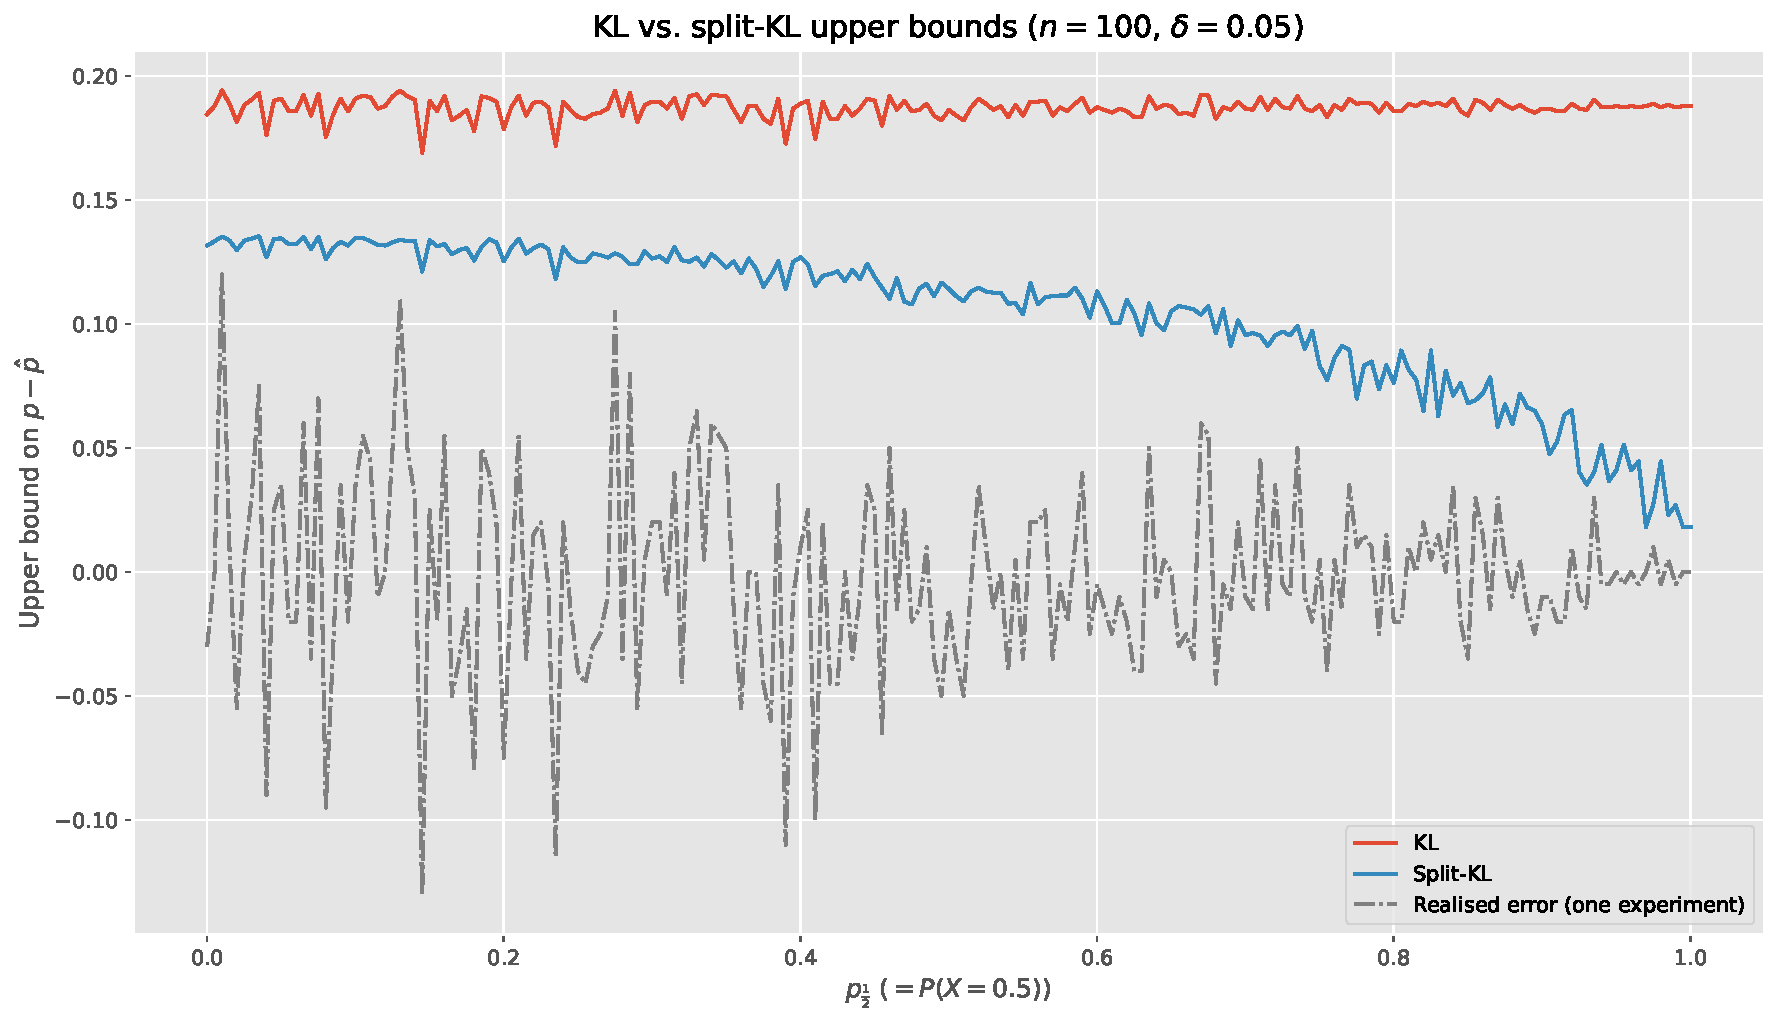
\includegraphics[scale=0.5]{figures/splitkl_vs_kl.pdf}
\label{fig:splitkl}
\end{figure}


\subsection*{Brief discussion}
Because the true mean is fixed at 0.5 for every choice of $p_{1/2}$, the empirical mean fluctuates around $0.5$, with variance depending on the shape of the distribution. 
\\[2mm]
The dashed curve is the error realized in the single sample that was drawn for each $p_{1/2}$
\\[2mm]
Let us consider what happens when $p_{\frac{1}{2}} \rightarrow 1$. In that case most of the probability mass is pushed to the center value 0.5, and the two outcomes (0 and 1) become very rare since their probabilities $p0 = p1 = (1-p_{\frac{1}{2}})/2 \rightarrow  0$. Consequently, the variance of X is given by $\Var(X)=0.25(1 -p_{\frac{1}{2}}) \rightarrow  0$. Hence the empirical mean is in practice locked very tightly around the true mean 0.5 once $p_{\frac{1}{2}}$ gets closer to 1.
\\[2mm]
Split-$\kl$ decomposes $X$ into the two binary indicators:
$$
X_{\mid 1} = \1[X \geq 0.5], \quad X_{\mid 2} = \1[X \geq 1].
$$
Their expectations are
\begin{align*}
    p_{\mid 1} &= \P(X \geq 0.5) = 1 - p_0  \rightarrow 1, \\
    p_{\mid 2} &= \P(X \geq 1.0) = p_1      \rightarrow 0
\end{align*}
as $p_{\frac{1}{2}} \rightarrow 1$.
\\[2mm]
When a Bernoulli parameter is very close to 0 or 1, the $\kl$-inverse difference $\klui(\hat{p},\epsilon)-\hat{p}$ is proportional to $\hat{p}(1-\hat{p})$ and therefore goes to zero.
\\[2mm]
For the split-$\kl$ bound these two tiny differences are multiplied by $\alpha_1 = \alpha_2 = 0.5$ and then added, so the whole bound collapses toward 0 as soon as $X$ almost never takes the extreme values.
That is why in figure \ref{fig:splitkl} we observe a split-$\kl$ close to 0 for $p_{\frac{1}{2}}$ close to 1.


\appendix

\section*{Python code}

\lstinputlisting[caption=Upper bound calculations, label={lst:upper_bounds}, language=python, style=myStyle]{code/upper_bounds.py}

\lstinputlisting[caption=Upper inverse, label={lst:upper_inverse}, language=python, style=myStyle]{code/upper_inverse.py}

\section*{Detailed calculation of quadratic roots}\label{sec:derivation}

Using the quadratic formula, the solutions to $aL^2 + bL + c = 0$ with
\begin{equation*}
a = 1, b = -\left(2\hat{L} + \frac{2\ln\frac{1}{\pi(h)\delta}}{n}\right), \,\text{and}\, c = \hat{L}^2
\end{equation*}
are:

$$L = \frac{\left(2\hat{L} + \frac{2\ln\frac{1}{\pi(h)\delta}}{n}\right) \pm \sqrt{\left(2\hat{L} + \frac{2\ln\frac{1}{\pi(h)\delta}}{n}\right)^2 - 4\hat{L}^2}}{2}$$

We simplify the discriminant:
\begin{align*}
\left(2\hat{L} + \frac{2\ln\frac{1}{\pi(h)\delta}}{n}\right)^2 - 4\hat{L}^2 &= 4\hat{L}^2 + \frac{8\hat{L}\ln\frac{1}{\pi(h)\delta}}{n} + \frac{4(\ln\frac{1}{\pi(h)\delta})^2}{n^2} - 4\hat{L}^2 \\
&= \frac{8\hat{L}\ln\frac{1}{\pi(h)\delta}}{n} + \frac{4(\ln\frac{1}{\pi(h)\delta})^2}{n^2}
\end{align*}

Hence the roots are:
$$L = \frac{2\hat{L} + \frac{2\ln\frac{1}{\pi(h)\delta}}{n} \pm \sqrt{\frac{8\hat{L}\ln\frac{1}{\pi(h)\delta}}{n} + \frac{4(\ln\frac{1}{\pi(h)\delta})^2}{n^2}}}{2}$$

Simplifying:
$$L = \hat{L} + \frac{\ln\frac{1}{\pi(h)\delta}}{n} \pm \sqrt{\frac{2\hat{L}\ln\frac{1}{\pi(h)\delta}}{n} + \frac{(\ln\frac{1}{\pi(h)\delta})^2}{n^2}}$$


%\bibliography{bibliography}  % If you have some references, use BibTeX

\end{document}
